\documentclass[tikz,border=12pt]{standalone}
\usepackage[T1]{fontenc}
\usepackage{mathpazo}
\usepackage{amsmath,amssymb}
\usetikzlibrary{arrows.meta, positioning, calc, fit, patterns, decorations.pathreplacing}

\definecolor{stblue}{HTML}{7B97AD}
\definecolor{rwgold}{HTML}{B8995E}
\definecolor{sage}{HTML}{7A9A7E}
\definecolor{dkbrown}{HTML}{3D3530}
\definecolor{wmgray}{HTML}{7B7067}
\definecolor{cream}{HTML}{F9F6F0}
\definecolor{border}{HTML}{D4C9B8}
\definecolor{terracotta}{HTML}{C47A6A}
\definecolor{lavender}{HTML}{907EA0}

\begin{document}
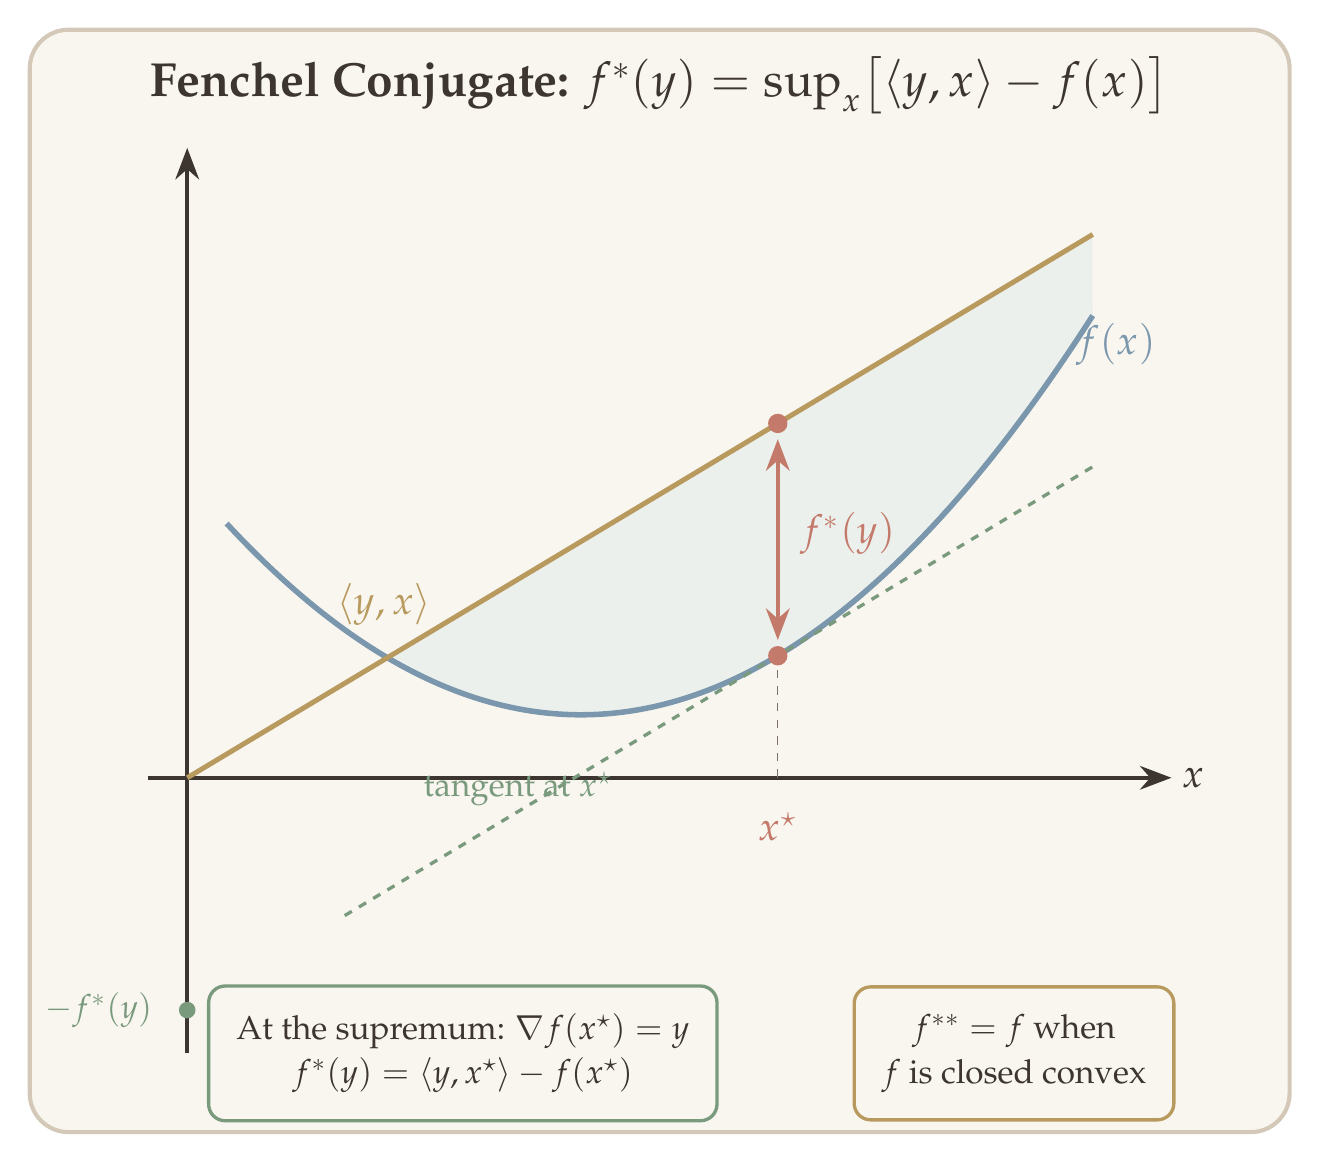
\begin{tikzpicture}[>={Stealth[length=4mm, width=3mm]}, line width=1.5pt]

% Background
\fill[cream, rounded corners=14pt] (-2,-4.5) rectangle (14,9.5);
\draw[border, line width=1.5pt, rounded corners=14pt] (-2,-4.5) rectangle (14,9.5);

% Title
\node[font=\LARGE\bfseries, text=dkbrown] at (6,8.8)
  {Fenchel Conjugate: $f^*(y) = \sup_x \bigl[\langle y, x\rangle - f(x)\bigr]$};

% f(x) = 0.12*(x-5)^2 + 0.8
% y = 0.6, line: t = 0.6x (through origin)
% x* = 7.5: f(7.5) = 1.55, line(7.5) = 4.5, f*(y) = 2.95
% Tangent at x*: t = 0.6x - 2.95, y-intercept = -f*(y) = -2.95

% --- Fills (drawn BEFORE axes) ---

% Shade gap region where line > f(x), x in [2.54, 11.5]
\fill[sage!15, smooth, samples=60]
  plot[domain=2.54:11.5] (\x, {0.6*\x})
  -- plot[domain=11.5:2.54] (\x, {0.12*(\x-5)*(\x-5) + 0.8})
  -- cycle;

% --- Axes ---
\draw[->, dkbrown, line width=1.5pt] (-0.5,0) -- (12.5,0)
  node[right, font=\Large, text=dkbrown] {$x$};
\draw[->, dkbrown, line width=1.5pt] (0,-3.5) -- (0,8)
  node[above, font=\Large, text=dkbrown] {};

% --- Curves and lines ---

% f(x) curve
\draw[stblue, line width=2pt, smooth, samples=80, domain=0.5:11.5]
  plot (\x, {0.12*(\x-5)*(\x-5) + 0.8});
\node[font=\Large, text=stblue] at (11.8,5.5) {$f(x)$};

% Linear function <y,x> = yx = 0.6x (through origin)
\draw[rwgold, line width=1.8pt, domain=0:11.5]
  plot (\x, {0.6*\x});
\node[font=\Large, text=rwgold] at (2.5,2.2) {$\langle y, x\rangle$};

% Tangent line at x* (same slope y, touches f at x*)
\draw[sage, line width=1.2pt, dashed, domain=2:11.5]
  plot (\x, {0.6*(\x - 7.5) + 1.55});
\node[font=\large, text=sage, above] at (4.2,-0.5) {tangent at $x^\star$};

% --- Points and gap ---

% Point on f(x) at x*
\fill[terracotta] (7.5, 1.55) circle (3.5pt);

% Point on line at x*
\fill[terracotta] (7.5, 4.5) circle (3.5pt);

% Gap arrow at x*: f*(y) = yx* - f(x*) = 4.5 - 1.55 = 2.95
\draw[terracotta, line width=1.5pt, <->] (7.5,1.75) -- (7.5,4.3);
\node[font=\Large\bfseries, text=terracotta, right] at (7.65,3.1) {$f^*(y)$};

% x* label on axis
\node[font=\Large, text=terracotta, below] at (7.5,-0.3) {$x^\star$};
\draw[wmgray, dashed, line width=0.5pt] (7.5,0) -- (7.5,1.4);

% y-intercept of tangent: -f*(y) = -2.95
\fill[sage] (0,-2.95) circle (3pt);
\node[font=\large, text=sage, left] at (-0.3,-2.95) {$-f^*(y)$};

% --- Annotation boxes ---
\node[fill=cream, draw=sage, line width=1.2pt, rounded corners=6pt,
      font=\large, text=dkbrown, align=center, inner sep=10pt]
  at (3.5,-3.5) {At the supremum: $\nabla f(x^\star) = y$\\[2pt]
  $f^*(y) = \langle y, x^\star \rangle - f(x^\star)$};

\node[fill=cream, draw=rwgold, line width=1.2pt, rounded corners=6pt,
      font=\large, text=dkbrown, align=center, inner sep=10pt]
  at (10.5,-3.5) {$f^{**} = f$ when\\[2pt] $f$ is closed convex};

\end{tikzpicture}
\end{document}
